%%%%%%%%%%%%%%%%%%%%%%%%%%%%%%%%%%%%%%%%%%%%%%%%%%%%%%%%%%%%%%%%%%%%%%%%%%%%%%
\documentclass[12pt,a4paper]{article}

%%%%%%%%%%%%%%%%%%%%%%%%%%%%%%%%%%%%%%%%%%%%%%%%%%%%%%%%%%%%%%%%%%%%%%%%%%%%%%
% Include a few packages

\usepackage{fontspec}
\setmainfont{TeX Gyre Heros}
\usepackage{hyperref}               % Hyperlinks
\usepackage[british]{babel}         % Use British English
\usepackage{graphicx}               % Graphics
\usepackage[svgnames,table]{xcolor} % Colours
\usepackage[hmargin=2cm,vmargin=2cm]{geometry} % Sort out the margins
\usepackage{tikz}                   % Graphics primitives
\usepackage{titlesec}               % Fancy section headings
\usepackage{pdfpages}               % Include pages from other PDFs
\usepackage{tabularx}               % Flexible tables

%%%%%%%%%%%%%%%%%%%%%%%%%%%%%%%%%%%%%%%%%%%%%%%%%%%%%%%%%%%%%%%%%%%%%%%%%%%%%%
% Package settings

% hyperref
\hypersetup{colorlinks=true, allcolors=black, pdftitle={BAMC 2023 Programme}} 

%%%%%%%%%%%%%%%%%%%%%%%%%%%%%%%%%%%%%%%%%%%%%%%%%%%%%%%%%%%%%%%%%%%%%%%%%%%%%%
% Styling

% Colours defined by the University of Bristol brand guidelines
\definecolor{UniversityRed}{RGB}{171, 31, 45}
\definecolor{CoolGrey}{RGB}{227, 230, 229}
\definecolor{BrightAqua}{RGB}{0, 192, 181}
\definecolor{BrightBlue}{RGB}{12, 198, 222}
\definecolor{BrightOrange}{RGB}{238, 114, 25}
\definecolor{BrightPurple}{RGB}{146, 120, 209}
\definecolor{BrightPink}{RGB}{224, 36, 154}
\definecolor{BrightLime}{RGB}{190, 214, 0}
\definecolor{DarkAqua}{RGB}{0, 67, 79}
\definecolor{DarkBlue}{RGB}{0, 47, 95}
\definecolor{DarkOrange}{RGB}{109, 38, 1}
\definecolor{DarkPurple}{RGB}{66, 20, 95}
\definecolor{DarkPink}{RGB}{119, 32, 89}
\definecolor{DarkLime}{RGB}{83, 104, 43}

% Paragraphs are separated by vertical space rather than indents
\setlength{\parindent}{0em}
\setlength{\parskip}{1.5ex plus 0.5ex minus 0.5ex}

% Where to find graphics
\graphicspath{{.}{./images/}}

% Remove section numbers
\setcounter{secnumdepth}{0}

% Format sections and subsections
\titleformat{\section}{\normalfont\LARGE\bfseries\scshape\color{UniversityRed}}{\thesection}{0.2em}{}
\titleformat{\subsection}{\normalfont\large\bfseries\color{DarkBlue}}{\thesubsection}{0.2em}{}
\newcommand{\sectionbreak}{\clearpage}

%\pagestyle{empty}

% New tabular column types for more control
\newcolumntype{Y}{>{\footnotesize\raggedright\arraybackslash}X}
\newcolumntype{P}[1]{>{\footnotesize\raggedright\let\newline\\\arraybackslash\hspace{0pt}}p{#1}}
\newcolumntype{C}[1]{>{\footnotesize\centering\let\newline\\\arraybackslash\hspace{0pt}}p{#1}}

%%%%%%%%%%%%%%%%%%%%%%%%%%%%%%%%%%%%%%%%%%%%%%%%%%%%%%%%%%%%%%%%%%%%%%%%%%%%%%
% Begin the text

\begin{document}
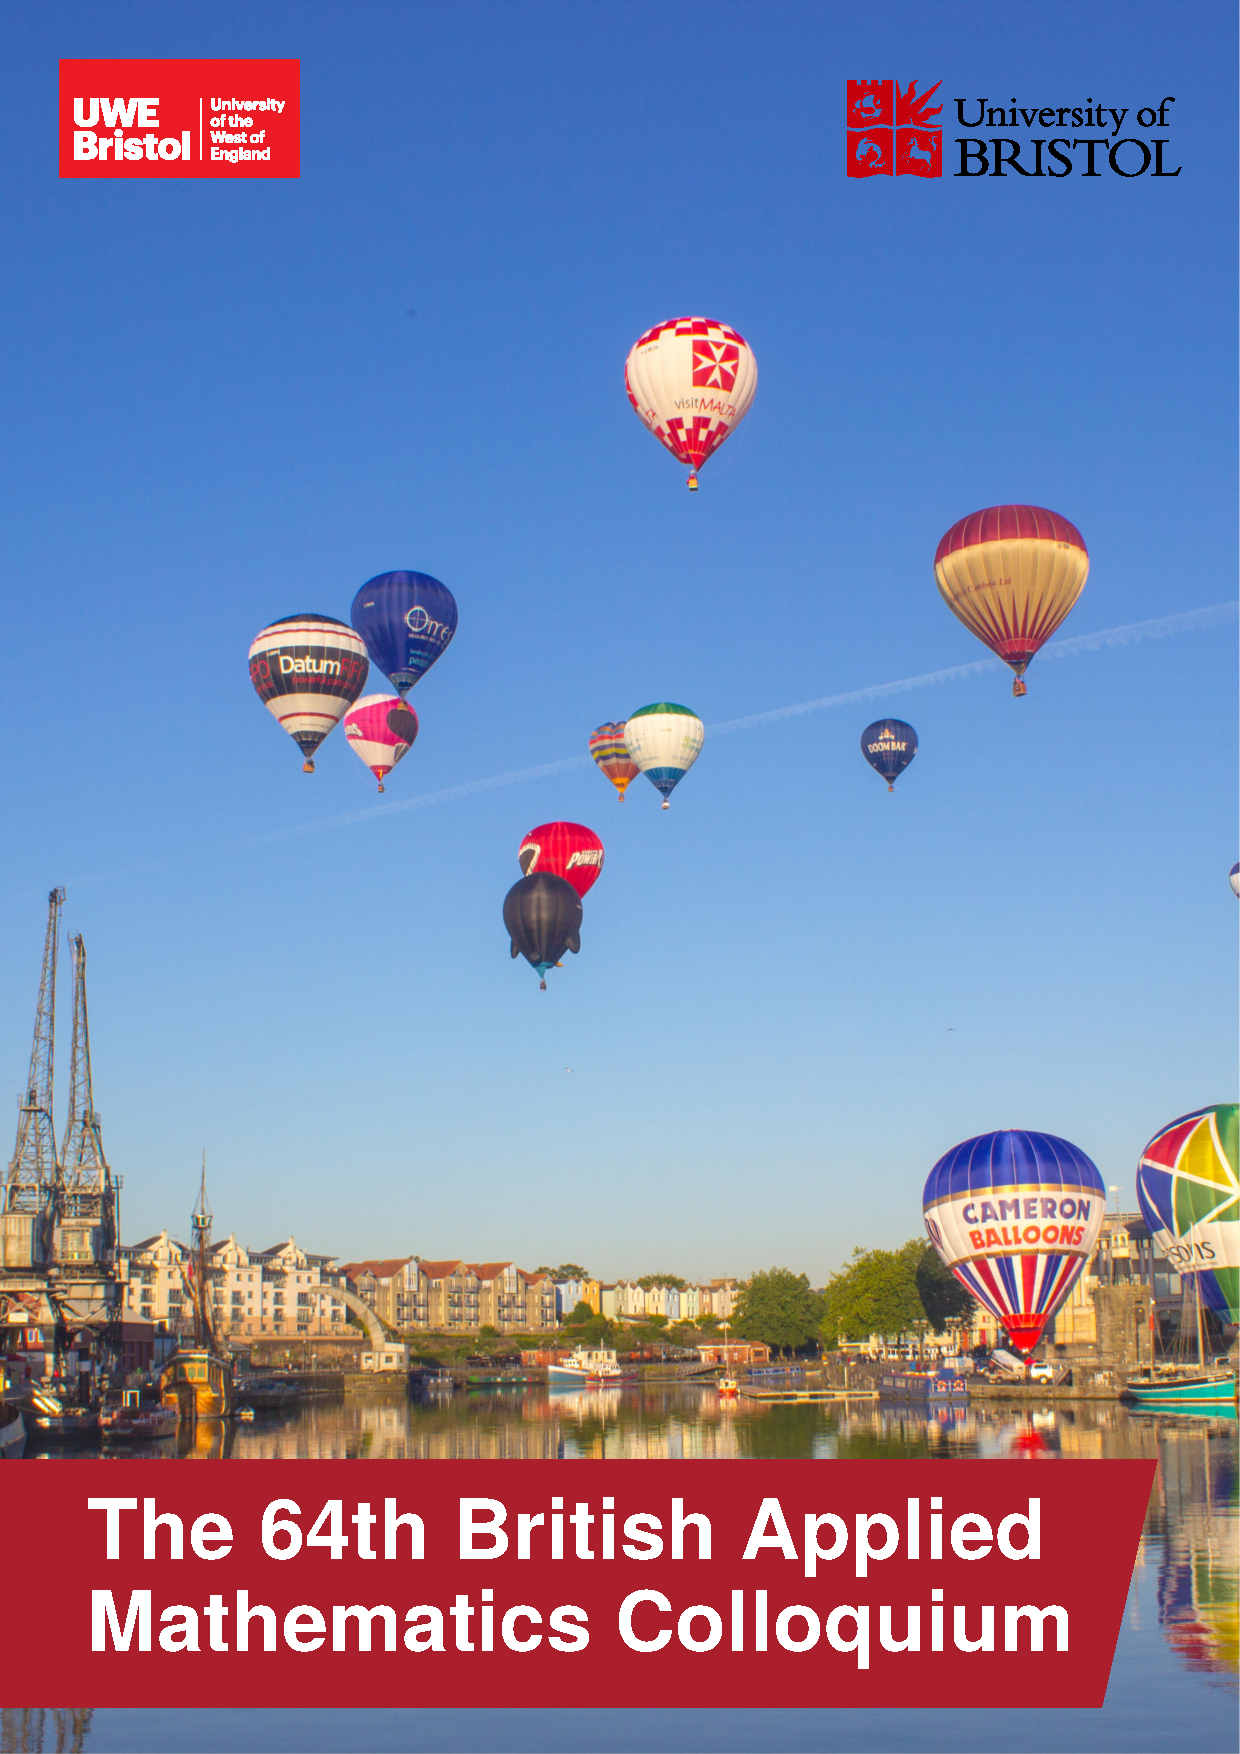
\includepdf{frontpage.pdf}
\setcounter{page}{1}

\section{Welcome}

\textcolor{DarkBlue}{\large Dear participants of the 64th BAMC, welcome to Bristol!}

The BAMC is a meeting that has a central place in the UK Applied Mathematics calendar. It is one of the first places where PhD students and Early Career Researchers present their work, and where mathematicians across all career stages have a chance to actively interact with each other.

\section{Essential Information}

\subsection{Website and latest information}

\subsection{Registration}

\subsection{Refreshments}

\subsection{Monday evening Poster Session and CUP wine reception}

\subsection{Conference Gala Dinner}

\subsection{Bars and pubs}

\subsection{Taxis}

\subsection{Parking on campus}

\subsection{Accommodation}

\subsection{Wi-Fi Access}

\section{Plenary Speakers}

\section{Programme Overview}

\section{Minisymposia Sessions}

\subsection{Monday 11:10–13:10}

\rowcolors{2}{BrightOrange!25}{BrightOrange!10}
\begin{tabularx}{\linewidth}{C{15mm}YP{50mm}}
\rowcolor{BrightOrange}\textcolor{white}{\textbf{2Q42}} & & \\
& \textbf{Advances in water waves and free-surface flows} & \\
11:10 & Water waves with vorticity and the Schwarz function & Darren Crowdy\\
11:30 & Exact solutions for submerged von Kármán point vortex streets cotravelling with a wave on a linear shear cuurent & Jack Keeler, Darren Crowdy\\
11:50 & On Ostrovsky-type models & Karima Khusnutdinova, Matthew Tranter\\
12:10 & Incipient wave breaking within higher-order spectral methods & Tatjana Kokina, J N Steer, S A Hasan, F Dias\\
12:30 & Desingularization and global continuation for hollow vortices & Miles Wheeler, Robin Ming Chen, Samuel Walsh\\
12:50 & Interfacial gravity waves and their limiting configurations & Xin Guan, Jean-Marc Vanden-Broeck\\
\end{tabularx}

\rowcolors{2}{BrightOrange!25}{BrightOrange!10}
\begin{tabularx}{\linewidth}{C{15mm}YP{50mm}}
\rowcolor{BrightOrange}\textcolor{white}{\textbf{2Q48}} & & \\
& \textbf{Mechanics of hydrogels and poroelastic media} & \\
11:10 & Multiscale modelling of a fibrous bioreactor scaffold & Amy Kent, James Oliver, Sarah Waters, Jon Chapman\\
11:30 & Formation and collapse of gas cavities in a soft porous medium & Oliver Paulin, Liam Morrow, Matthew Hennessy, Christopher MacMinn\\
11:50 & Multiple scales homogenisation of a porous viscoelastic material with rigid inclusions & Andres F Galvis, J M Foster, Bartosz Protas, Stephen J Chapman\\
12:10 & Swelling-induced folds in soft microchannels & Haolin Li, Aidan Retallick, Anne Juel, Matthias Heil, Draga Pihler-Puzovic\\
12:30 & Computational Modelling of stimuli-responsive hydrogels & Amin Rahmat, Mostafa Safdari Shadloo, Tom Montenegro-Johnson\\
12:50 & Curvature-controlled beading in stretched hydrogel cylinders & Matteo Taffetani, Matthew Hennessy\\
\end{tabularx}

\rowcolors{2}{BrightOrange!25}{BrightOrange!10}
\begin{tabularx}{\linewidth}{C{15mm}YP{50mm}}
\rowcolor{BrightOrange}\textcolor{white}{\textbf{2Q49}} & & \\
& \textbf{Dynamics of reaction-transport systems} & \\
11:10 & VisualPDE: Using WebGL to Rapidly Explore PDE Dynamics for Fun and Profit & Andrew Krause, Benjamin Walker, Adam Townsend\\
11:50 & Reaction-Transport Dynamics in the Decontamination of Porous Media & Ellen Luckins\\
12:10 & Pattern Formation in a Nonlocal Model for Cell Attraction and Repulsion in 2 or More Dimensions & Thomas Jun Jewell, Andrew L Krause, Philip K Maini, Eamonn A Gaffney\\
12:30 & Pattern formation in multiphase, moving boundary models of tissue growth & Jacob Jepson, John Billingham, Reuben O'Dea, Nabil Fadai\\
12:50 & Minimal reaction schemes for Turing instabilities & Fraser Waters, Kit Yates, Jonathan Dawes\\
\end{tabularx}

\rowcolors{2}{BrightOrange!25}{BrightOrange!10}
\begin{tabularx}{\linewidth}{C{15mm}YP{50mm}}
\rowcolor{BrightOrange}\textcolor{white}{\textbf{2Q50/51}} & & \\
& \textbf{How to be better prepared for a future pandemic: lessons learned from COVID-19, mpox and the four historic influenza pandemics} & \\
11:10 & Importance of progressive transmissibility of emerging variants in sustaining the COVID-19 epidemic in England & Ben Swallow\\
11:30 & The interplay between population susceptibility and vaccine effectiveness control the timing and size of an emerging influenza wave & Edwin Van Leeuwen\\
11:50 & Considerations for informing Test, Trace and support to Isolate (TTI) intervention design following the experience of COVID-19 & Elizabeth Fearon\\
12:10 & The role of enclosed population in an epidemic  & Thomas Finnie\\
12:30 & WasteWater as a pandemic surveillance tool & Zhou Fang\\
12:50 & Lessons from modelling during a pandemic and for pandemic preparedness  & Jasmina Panovska-Griffiths\\
\end{tabularx}

\rowcolors{2}{BrightOrange!25}{BrightOrange!10}
\begin{tabularx}{\linewidth}{C{15mm}YP{50mm}}
\rowcolor{BrightOrange}\textcolor{white}{\textbf{4Q56}} & & \\
& \textbf{Physiological flows and transport} & \\
11:10 & Generalised tube laws for the deformation of elastic-walled tubes with arbitrary cross-sections & Daniel Netherwood, Robert J Whittaker\\
11:30 & Understanding the mechanism of unconventional drainage from the eye & Jennifer Tweedy, Mariia Dvoriashyna, Jessica Crawshaw, Darryl Overby, Rodolfo Repetto, Paul Roberts, Tamsin Spelman, Peter Stewart, Alexander Foss\\
11:50 & Modelling oxygen transport in the human cerebral microvasculature & Yidan Xue, Stephen Payne\\
12:10 & Modelling metabolite transport in hollow fibre membrane bioreactors & George Booth, Mohit Dalwadi, Pierre-Alexis Mouthuy, Hua Ye, Sarah Waters\\
12:30 & Flow and transport in the human placenta: from multiscale imaging to structural determinants of function & Igor Chernyavsky, Alys Clark, Alexander Erlich, Oliver Jensen, Philip Pearce, Win Tun, Carl Whitfield, et al.\\
12:50 & Oscillatory and steady streaming flow of cerebrospinal fluid during the cardiac cycle & Mariia Dvoriashyna, Alain Goriely\\
\end{tabularx}

\subsection{Monday 14:10–16:10}

\rowcolors{2}{BrightOrange!25}{BrightOrange!10}
\begin{tabularx}{\linewidth}{C{15mm}YP{50mm}}
\rowcolor{BrightOrange}\textcolor{white}{\textbf{2Q42}} & & \\
& \textbf{Advances in water waves and free-surface flows} & \\
14:10 & Modulational instability and recurrence of hydrodynamic waves with frequency-dependent dissipation & Alberto Alberello, Emilian Parau\\
14:30 & A thin plate approximation for thick floating ice & Luke Bennetts\\
14:50 & Ship wave patterns on floating ice sheets & Emilian Parau\\
15:10 & The nonlinear Benjamin-Feir instability - a discrete Hamiltonian approach & Raphael Stuhlmeier, David Andrade\\
15:30 & Exponential asymptotics for the Saffman-Taylor problem in a wedge & Cecilie Andersen, Chris Lustri, Scott McCue, Phil Trinh\\
15:50 & Three dimensional hydroelastic solitary waves  in shallow water & Yanghan Meng, Zhan Wang\\
\end{tabularx}

\rowcolors{2}{BrightOrange!25}{BrightOrange!10}
\begin{tabularx}{\linewidth}{C{15mm}YP{50mm}}
\rowcolor{BrightOrange}\textcolor{white}{\textbf{2Q48}} & & \\
& \textbf{Controlling active matter} & \\
14:10 & Odd dynamics of living chiral crystals & Alexander Mietke, T H Tan, J Li, Y Chen, H Higinbotham, P J Foster, S Gokhale, J Dunkel, N Fakhri\\
14:30 & Conditions for hydrodynamic coordination in arrays of model cilia & Rachel Bennett, Fanlong Meng, Nariya Uchida, Ramin Golestanian\\
14:50 & Is the tendency for all living systems to do work universal? & Elsen Tjhung\\
15:10 & Shear thickening and Yielding Transitions in Biological Tissues & Michael Hertaeg, Suzanne Fielding, Dapeng Bi\\
15:30 & Active elastocapillarity in soft solids with negative surface tension & Jack Binysh, Thomas R Wilks, Anton Souslov\\
15:50 & Large deviations and optimal control in active fluids & Robert Jack\\
\end{tabularx}

\rowcolors{2}{BrightOrange!25}{BrightOrange!10}
\begin{tabularx}{\linewidth}{C{15mm}YP{50mm}}
\rowcolor{BrightOrange}\textcolor{white}{\textbf{2Q49}} & & \\
& \textbf{Dynamics of reaction-transport systems} & \\
14:10 & Pattern Formation on a Finite Disk, Variational and Non Variational Case & Nicolas Verschueren van Rees, Edgar Knobloch, Hannes Uecker\\
14:30 & Understanding fully localised 2D patterns with dihedral symmetry & Dan J Hill, Jason J Bramburger, David J B Lloyd\\
14:50 & Homoclinic snaking \& localised patterns beyond all asymptotic orders & Edgardo Villar-Sepúlveda, Alan Champneys\\
15:10 & Nonlocal models of cell-cell adhesion and their Cahn-Hilliard approximation & Carles Falcó, Ruth E Baker, José A Carrillo\\
15:30 & Stability and multi-stability in non-local advection-diffusion models & Valeria Giunta, Thomas Hillen, Mark Lewis, Jonathan Potts\\
15:50 & Self-organised patterning in Dictyostelium group migration & Giulia Celora, Hugh Ford, Mohit Dalwadi, Benjamin Walker, Jonathan Chubb, Philip Pearce\\
\end{tabularx}

\rowcolors{2}{BrightOrange!25}{BrightOrange!10}
\begin{tabularx}{\linewidth}{C{15mm}YP{50mm}}
\rowcolor{BrightOrange}\textcolor{white}{\textbf{2Q50/51}} & & \\
& \textbf{Mathematical pharmacology} & \\
14:10 & Practical application of quantitative systems toxicology models in drug development: learnings and case studies from the IMI2-tQST project & Ciarán Fisher\\
14:50 & Extensions of receptor theory to include dimerised and dimerising receptor dynamics & Lloyd Bridge, Carla White\\
15:10 & Physiologically-Based Pharmacokinetic Modelling: The Double-Edged Sword of Complexity & Aleksandra Kmieciak\\
15:30 & Cybergenetics applications in mammalian cells: closing the loop on non-linear dynamics & Lucia Marucci\\
15:50 & Structural Identifiability Analysis: A Tool for Mathematical Pharmacology & Michael Chappell, Neil D Evans\\
\end{tabularx}

\rowcolors{2}{BrightOrange!25}{BrightOrange!10}
\begin{tabularx}{\linewidth}{C{15mm}YP{50mm}}
\rowcolor{BrightOrange}\textcolor{white}{\textbf{4Q56}} & & \\
& \textbf{Mathematical and computational ophthalmology} & \\
14:10 & Mathematical and Computational Ophthalmology: Coming of Age & Paul A Roberts\\
14:30 & A tool for automated retinal vascular morphology quantification and its applications & Yukun Zhou, Daniel Alexander, Pearse Keane\\
14:50 & Pressure wave transmission across the lamina cribrosa & Peter Stewart, Ifeanyi Sunday Onah, David MacTaggart\\
15:10 & High amplitude elastic jump propagation through blood vessel junctions  & Tamsin A Spelman, Ifeanyi S Onah, David MacTaggart, Peter S Stewart\\
15:30 & Characterising eyes with neovascular age-related macular degeneration & Remi Hernandez\\
15:50 & The important role of hierarchical Bayesian inference in understanding macular degeneration treatment strategies & Jessica Crawshaw, Eamonn Gaffney, Philip Maini, Antonello Caruso, Michael Gertz\\
\end{tabularx}

\subsection{Tuesday 10:30–12:30}

\rowcolors{2}{BrightBlue!25}{BrightBlue!10}
\begin{tabularx}{\linewidth}{C{15mm}YP{50mm}}
\rowcolor{BrightBlue}\textcolor{white}{\textbf{2Q42}} & & \\
& \textbf{Mathematical modelling in sport} & \\
10:30 & Gunwale bobbing and the effect of heave and pitch during a rowing race & Graham P Benham\\
10:50 & Improving the self-stability of a bicycle via spectral abscissa minimisation & Oleg Kirillov\\
11:10 & Effects of friction and tangential compliance in golf ball bounce & Stanislaw W Biber, Alan R Champneys, Robert Szalai\\
11:30 & Alpine pendulum & Serguei Komissarov\\
11:50 & Analysis of Soccer Ball Collision Kinematics and Kinetics Using Image Processing Techniques & Ieuan Phillips, Andy Harland, Séan Mitchell, Paul Lepper\\
12:10 & Exploration into the spatial and temporal movement of the female breast during motion. & Lauren Holmes, Andy Harland\\
\end{tabularx}

\rowcolors{2}{BrightBlue!25}{BrightBlue!10}
\begin{tabularx}{\linewidth}{C{15mm}YP{50mm}}
\rowcolor{BrightBlue}\textcolor{white}{\textbf{2Q48}} & & \\
& \textbf{Advances in applied numerical linear algebra and its applications} & \\
10:30 & Flexible and inexact Krylov methods for inverse problems & Malena Sabaté Landman\\
11:10 & Applied Krylov subspace algorithms in CT using the TIGRE toolbox & Ander Biguri, Malena Sabate Landman, Sepideh Hatamikia, Richard Boardman, John Aston, Carola-Bibiane Schonlieb\\
11:30 & Structure-Exploiting Preconditioners for Data Assimilation & Jemima Tabeart, John W Pearson, Selime Gürol, Anthony Weaver\\
11:50 & Model Based Iterative Reconstruction of Tomographic data with the Core Imaging Library & Edoardo Pasca, Evelina Ametova, Gemma Fardell, Jakob Sauer Jørgensen, Laura Murgatroyd, Evangelos Papoutsellis\\
12:10 & Data-Driven Mirror Descent with Input-Convex Neural Networks & Subhadip Mukherjee, Hong Ye Tan, Junqi Tang, Andreas Hauptmann, Carola-Bibiane Schönlieb\\
\end{tabularx}

\rowcolors{2}{BrightBlue!25}{BrightBlue!10}
\begin{tabularx}{\linewidth}{C{15mm}YP{50mm}}
\rowcolor{BrightBlue}\textcolor{white}{\textbf{2Q49}} & & \\
& \textbf{IMA Lighthill-Thwaites prize} & \\
10:50 & Modelling melting, structure and microbial activity of an ice sheet surface & Tilly Woods, Ian Hewitt\\
11:10 & Exponential asymptotics for steady capillary ripples on steep gravity waves & Josh Shelton\\
11:30 & On the deformation of an elastic particle under pressure-driven axisymmetric channel flow & Simon M Finney, Matthew G Hennessy, Andreas Muench, Sarah Waters\\
11:50 & Matched asymptotics, conformal capacity, and applications & Hiroyuki Miyoshi, Darren G Crowdy\\
12:10 & Controlling stratification in drying films with diffusiophoresis & Clare Rees-Zimmerman, Alex Routh\\
\end{tabularx}

\rowcolors{2}{BrightBlue!25}{BrightBlue!10}
\begin{tabularx}{\linewidth}{C{15mm}YP{50mm}}
\rowcolor{BrightBlue}\textcolor{white}{\textbf{2Q50/51}} & & \\
& \textbf{Neurodynamics} & \\
10:30 & Modeling Alzheimer's progression: Oscillator dynamics on evolving networks & Christoffer Gretarsson Alexandersen, Alain Goriely, Christian Bick, Willem de Haan\\
10:50 & Phase-Isostable Reduction of Coupled Oscillator Networks & Robert Allen\\
11:10 & Exploring the bifurcations of excitable cells with control-based continuation & Mark Blyth, Krasimira Tsaneva-Atanasova, Kyle Wedgwood, Lucia Marucci, Ludovic Renson\\
11:30 & Tonic-clonic seizure transitions in a next generation neural field model & Oliver Cattell\\
11:50 & Hierarchical processing underpins competition in tactile perceptual bistability & Farzaneh Darki, Andrea Ferrario, James Rankin\\
12:10 & Investigating travelling waves in a 2D network of spiking neurons & Henry Kerr\\
\end{tabularx}

\rowcolors{2}{BrightBlue!25}{BrightBlue!10}
\begin{tabularx}{\linewidth}{C{15mm}YP{50mm}}
\rowcolor{BrightBlue}\textcolor{white}{\textbf{4Q05}} & & \\
& \textbf{Multiple wave scattering} & \\
10:30 & Multiple scattering in the spirit of Leslie Foldy & Paul Martin\\
11:10 & High-frequency homogenization for dispersive materials of the Lorentz type & Marie Touboul, R Assier, R Craster, S Guenneau, B Vial\\
11:30 & Diffraction by a finite barrier/crack on a square lattice: an iterative Wiener-Hopf method approach & Elena Medvedeva, Anastasia Kisil, Raphael Assier\\
11:50 & Effects of gravity and dispersive waves in chiral elastic systems & Alessio Kandiah, Ian S Jones, Natasha V Movchan, Alexander B Movchan\\
12:10 & Time-dependent problems in Wave Scattering & Michael Meylan\\
\end{tabularx}

\rowcolors{2}{BrightBlue!25}{BrightBlue!10}
\begin{tabularx}{\linewidth}{C{15mm}YP{50mm}}
\rowcolor{BrightBlue}\textcolor{white}{\textbf{4Q56}} & & \\
& \textbf{Chemo-mechanical couplings in growing tissues} & \\
10:30 & A patient-specific framework for studying the influence of chemo-mechanical cues on brain tumour growth and surrounding healthy tissue damage. & Chiara Giverso, Francesca Ballatore, Giulio Lucci\\
11:10 & Minimal Morphoelastic Models of Solid Tumour Spheroids & Benjamin Walker, Giulia L Celora, Alain Goriely, Derek E Moulton, Helen M Byrne\\
11:30 & The effects of non-local diffusion on the growth of an avascular tumour & Ariel Ramirez Torres, Mariam Al Mudarra, Alfio Grillo\\
11:50 & Mechanotransduction in axon: Remodelling of the actin cortex & Davide Riccobelli, D Andrini, V Balbi, G Bevilacqua, G Lucci, G Pozzi\\
12:10 & Mechanical feedback in size regulation & Alexander Erlich, Pierre Recho\\
\end{tabularx}

\subsection{Tuesday 13:30–15:30}

\rowcolors{2}{BrightBlue!25}{BrightBlue!10}
\begin{tabularx}{\linewidth}{C{15mm}YP{50mm}}
\rowcolor{BrightBlue}\textcolor{white}{\textbf{2Q42}} & & \\
& \textbf{Sea ice modelling} & \\
13:30 & From Micro to Macro in Sea Ice Modelling & Kenneth M Golden\\
14:10 & Partial Differential Equation Models and Deep Learning for the Sea Ice Concentration Field & Delaney Mosier\\
14:30 & Seasonal evolution of the Arctic sea ice thickness distribution & Srikanth Toppaladoddi, Woosok Moon, John S Wettlaufer\\
14:50 & A computational model of the freezing of salt water  & Brian Wetton\\
15:10 & Dynamics of Brine Inclusions in First Year Sea Ice & Keith Promislow, Noa Kraitzman, Yuan Chen, Brian Wetton\\
\end{tabularx}

\rowcolors{2}{BrightBlue!25}{BrightBlue!10}
\begin{tabularx}{\linewidth}{C{15mm}YP{50mm}}
\rowcolor{BrightBlue}\textcolor{white}{\textbf{2Q49}} & & \\
& \textbf{IMA Lighthill-Thwaites prize} & \\
13:30 & Nonlinear waves in viscous multilayer shear flows in the presence of interfacial slip & Anna Katsiavria, Demetrios T Papageorgiou\\
13:50 & A two-complex-variable approach to the right-angled no-contrast penetrable wedge diffraction problem & Valentin Kunz, Raphael Assier\\
14:10 & Data-driven discovery of PDEs & Nicolas Boullé, Alex Townsend\\
\end{tabularx}

\rowcolors{2}{BrightBlue!25}{BrightBlue!10}
\begin{tabularx}{\linewidth}{C{15mm}YP{50mm}}
\rowcolor{BrightBlue}\textcolor{white}{\textbf{2Q50/51}} & & \\
& \textbf{Modelling and inference in public health} & \\
13:30 & Bayesian multilevel modelling for prediction and uncertainty estimation of motor progression in Parkinson's disease & Tanja Zerenner, Michael Lawton, Anahita Nodehi, Donald Grosset \& the Tracking Parkinson’s team, Michele Hu \& the OPDC-Discovery team, Yoav Ben-Shlomo\\
13:50 & The role of large connected components in sexual networks for HIV spreading in Sub-Saharan Africa & Francesco Di Lauro\\
14:10 & How data-driven, mechanistic modelling is being used to support elimination of African sleeping sickness  & Kat S Rock\\
14:30 & Combining models to generate consensus nowcasts for the COVID-19 epidemic status in England & Harrison Manley, Josie Park, Luke Bevan, Alberto Sanchez-Marroquin, Gabriel Danelian, Thomas Bayley, Veronica Bowman, Thomas Maishman, Thomas Finnie, Andre Charlett, Nicholas A Watkins, Johanna Hutchinson, Steven Riley, Jasmina Panovska-Griffiths, Sebastian Funk, Paul Birrell, Daniela De Angelis, Matt Keeling, Lorenzo Pellis, Marc Baguelin, Graeme Ackland, Jonathan Read, Christopher Jewell, Robert Challen\\
14:50 & The observational model: a data-driven parameter estimation technique for dynamical systems & James Van Yperen, Eduard Campillo-Funollet, Anotida Madzvamuse\\
\end{tabularx}

\rowcolors{2}{BrightBlue!25}{BrightBlue!10}
\begin{tabularx}{\linewidth}{C{15mm}YP{50mm}}
\rowcolor{BrightBlue}\textcolor{white}{\textbf{4Q05}} & & \\
& \textbf{Multiple wave scattering} & \\
13:30 & Full Waveform Inversion via Reduced Order Modeling & Josselin Garnier, Liliana Borcea, Alexander Mamonov, Jorn Zimmerling\\
13:50 & Wave Scattering from Layers of Random Particulate Materials & Paulo Sergio Piva, Kevish K Napal, Artur L Gower\\
14:10 & Using elastic waves to predict forces in thick-walled cylinder with application to roller-bearings & Jessica Jordan Kent, Artur Lewis Gower\\
14:30 & Causality Constraint as a Design Tool for Sound Absorption Metastructures & Ping Sheng\\
14:50 & Multiple wave scattering in soft complex media & Valerie J Pinfield\\
15:10 & Spectral convergence of defect modes in large finite resonator arrays & Bryn Davies\\
\end{tabularx}

\rowcolors{2}{BrightBlue!25}{BrightBlue!10}
\begin{tabularx}{\linewidth}{C{15mm}YP{50mm}}
\rowcolor{BrightBlue}\textcolor{white}{\textbf{4Q56}} & & \\
& \textbf{New mathematical approaches in the life sciences} & \\
13:30 & Exploring electrical environments: the unique sense of electroreception & Ryan Palmer, Isaac V Chenchiah, Daniel Robert\\
13:50 & Extended Pair Correlation Functions for Multiplex Medical Imaging & Joshua A Bull, Helen M Byrne\\
14:10 & Mathematics, the Mind and Alzheimer's disease: Systematical progression on brain graphs & Prama Putra, Alain Goriely\\
14:30 & Field Theories of Branching in Cell Populations, Epidemiology and Neuronal Signals & Johannes Pausch\\
14:50 & Viral geometry as a key to understanding viral infections & Reidun Twarock\\
15:10 & Mathematical and deep learning analysis of wound healing in flies & Jake Turley, I V Chenchiah, T B Liverpool, H Weavers, P Martin\\
\end{tabularx}

\subsection{Wednesday 10:30–12:30}

\rowcolors{2}{BrightPurple!25}{BrightPurple!10}
\begin{tabularx}{\linewidth}{C{15mm}YP{50mm}}
\rowcolor{BrightPurple}\textcolor{white}{\textbf{2Q42}} & & \\
& \textbf{Mathematical modelling of sleep and circadian rhythms: from molecular mechanisms to policy} & \\
10:30 & Mathematical modelling of the wheat circadian clock & Abhishek Upadhyay, Jamila Rowland-Chandler, Gabriela Pingarron-Cardenas, Alex Webb, James Locke\\
10:50 & Modelling the cell-autonomous lung circadian clock & Matthew Leak\\
11:10 & Ticking and talking in the brainstem satiety centre: A phase model of three clocks     & Jake Ahern, Lukasz Chrobok, Hugh Piggins, Alan Champneys\\
11:30 & TimeTeller: a tool to analyse from data the circadian clock as a multigene dynamical system. & David Rand\\
11:50 & Regulation of human sleep timing and physiology by biological oscillators coding for history and time and influenced by environmental cycles & Derk-Jan Dijk\\
12:10 & Maths, sleep and policies for 21st century living & Anne Skeldon\\
\end{tabularx}

\rowcolors{2}{BrightPurple!25}{BrightPurple!10}
\begin{tabularx}{\linewidth}{C{15mm}YP{50mm}}
\rowcolor{BrightPurple}\textcolor{white}{\textbf{2Q48}} & & \\
& \textbf{Optimisation and control for nonlinear dynamics} & \\
10:30 & Optimisation and control for nonlinear dynamics & Susana Gomes, Dante Kalise\\
11:10 & Falling liquid film control via linear quadratic regulation & Oscar Holroyd, Susana N Gomes, Radu Cimpeanu\\
11:30 & Computational Modelling and Optimal Control for Interacting Particle Systems & Jonna Roden\\
11:50 & Supervised learning control of kinetic collective dynamics & Sara Bicego, Dante Kalise, Giacomo Albi\\
12:10 & Oblique projections for state estimation and state stabilization of parabolic-like systems & Sergio S Rodrigues\\
\end{tabularx}

\rowcolors{2}{BrightPurple!25}{BrightPurple!10}
\begin{tabularx}{\linewidth}{C{15mm}YP{50mm}}
\rowcolor{BrightPurple}\textcolor{white}{\textbf{2Q49}} & & \\
& \textbf{Networks and complex systems in society} & \\
10:30 & SHEEP: Signed Hamiltonian Eigenvector Embedding for Proximity & Shazia Babul\\
10:50 & Mitigating the impact of negative vaccine-related information diffusion & Sarah Alahmadi, Rebecca Hoyle, Markus Brede\\
11:10 & Binary Synchronization of Randomly Forced Oscillators & Jeremy Worsfold\\
11:30 & Enabling Imitation-Based Cooperation in Dynamic Social Networks & Jacques Bara, Paolo Turrini, Giulia Andrighetto\\
11:50 & Analysing The Uncertainty of Wiretaps in Criminal Networks & Daniel Catlin\\
12:10 & Modelling Social Dynamics on Clustered Networks & Leah Keating\\
\end{tabularx}

\rowcolors{2}{BrightPurple!25}{BrightPurple!10}
\begin{tabularx}{\linewidth}{C{15mm}YP{50mm}}
\rowcolor{BrightPurple}\textcolor{white}{\textbf{4Q05}} & & \\
& \textbf{Metamaterial modelling and design} & \\
10:30 & Homogenization of Irrational Metamaterials: Two-Scale Cut-and-Projection Method & Sebastien Guenneau, Elena Cherkaev, Niklas Wellander, Frederic Zolla\\
11:10 & The inverse design of disordered metamaterials using the coupled dipole framework & James Capers\\
11:30 & Wave interaction with subwavelength resonators & Jinghao Cao\\
11:50 & A Photonic Crystal of Metacylinder Inclusions  & Henry Putley, Sebastien Guenneau, Richard Craster\\
12:10 & Failure by design of confined architected interfaces & Adrianos E F Athanasiadis, Michal K Budzik, Dilum N Fernando, Marcelo A Dias\\
\end{tabularx}

\rowcolors{2}{BrightPurple!25}{BrightPurple!10}
\begin{tabularx}{\linewidth}{C{15mm}YP{50mm}}
\rowcolor{BrightPurple}\textcolor{white}{\textbf{4Q56}} & & \\
& \textbf{Asymptotics in active matter} & \\
10:30 & Emergent three-dimensional dynamics of rapidly spinning, self-propelled chiral particles in shear flow & Mohit Dalwadi, Clément Moreau, Eamonn Gaffney, Benjamin Walker, Kenta Ishimoto\\
10:50 & Modelling the transport of active particles in a dilute suspension & Lloyd Fung, R N Bearon, Y Hwang\\
11:10 & Stability in an active exclusion process & James Mason, Maria Bruna, Rob L Jack, Clement Erignoux\\
11:30 & Weakly nonlinear dynamics of self-propelling active particles & Gunnar Peng, Ory Schnitzer\\
11:50 & Motility-Induced Phase Separation in Signalling Bacteria & Wesley Ridgway\\
12:10 & Beyond Slender-body theory  & Lyndon Koens\\
\end{tabularx}



\section{Contributed Talks Sessions}

\section{Poster Presentation}

\section{Sponsors, Funders, and Exhibitors}

\section{Map}

\end{document}
